\subsubsection{Visual Analysis of \ce{SiO_2} Distribution in Folds}
This section aims to provide a detailed visualization and statistical analysis of the \ce{SiO_2} concentration distribution across different folds used in our custom k-fold data partitioning procedure.
The purpose is to demonstrate the effectiveness of our strategy in maintaining balanced and representative datasets, which is crucial for developing robust predictive models.

We focus specifically on \ce{SiO_2} as a representative example to illustrate our methodology.
Similar analyses were conducted for other oxides; however, the plots and figures for these are omitted here for brevity.

Figure \ref{fig:histogram_grid_plot} presents individual histograms and \gls{kde} curves for \ce{SiO_2} concentrations in each of the four cross-validation folds' validation sets and the full test set.
The overlaid \gls{kde} curves provide a smoothed estimate of the probability density function for \ce{SiO_2} concentrations.

\begin{figure*}[h!]
    \centering
    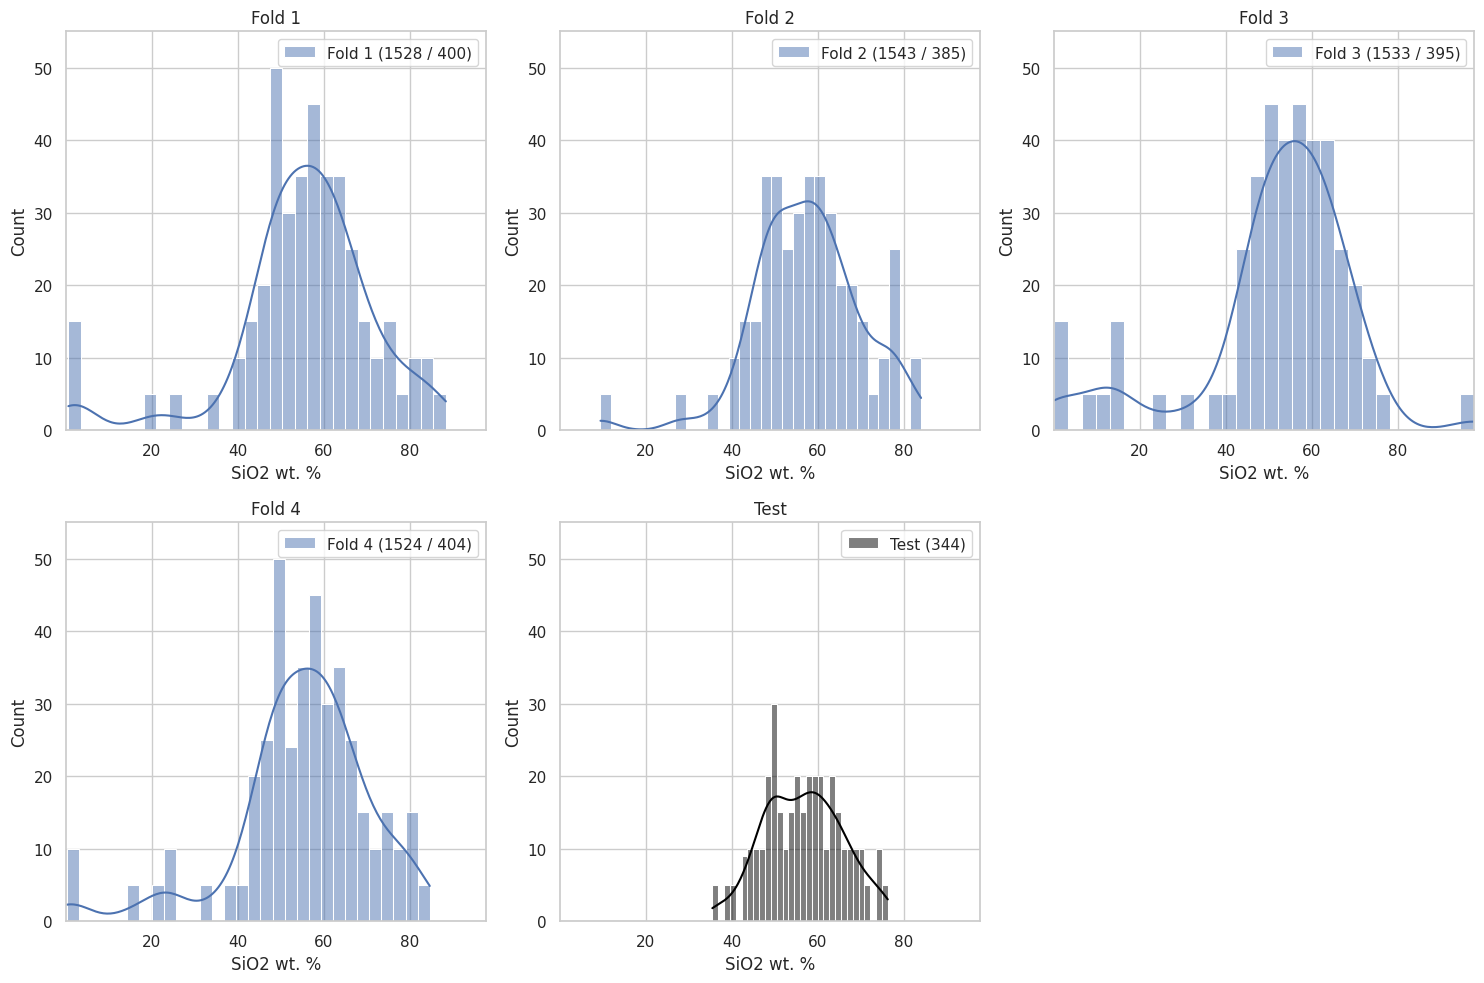
\includegraphics[width=\textwidth]{images/histogram_grid_plot.png}
    \caption{Histogram and \gls{kde} of \ce{SiO_2} Distribution in Each Fold. The y-axis represents the count of samples per bin, and the x-axis represents \ce{SiO_2} concentration. The notation in the legend indicates the amount of instances in the training/validation sets.}
    \label{fig:histogram_grid_plot}
\end{figure*}

The histograms and \gls{kde} curves for each fold are remarkably similar, indicating that the data distribution within each fold closely matches the overall data distribution.
This similarity ensures that each fold is representative of the entire dataset, which is crucial for developing models that can generalize well.
The central tendency (mean) and spread (standard deviation) of \ce{SiO_2} concentrations appear consistent across all folds.
The \gls{kde} curves highlight that the density peaks and the tails of the distributions align well, suggesting that no fold is disproportionately skewed or biased.

These consistent distributions across folds validate our k-fold data partitioning method, confirming that each fold can provide a reliable estimate of model performance.
This balance helps in preventing overfitting, as the model is trained and validated on similarly distributed data in each fold.

\begin{figure*}[h!]
    \centering
    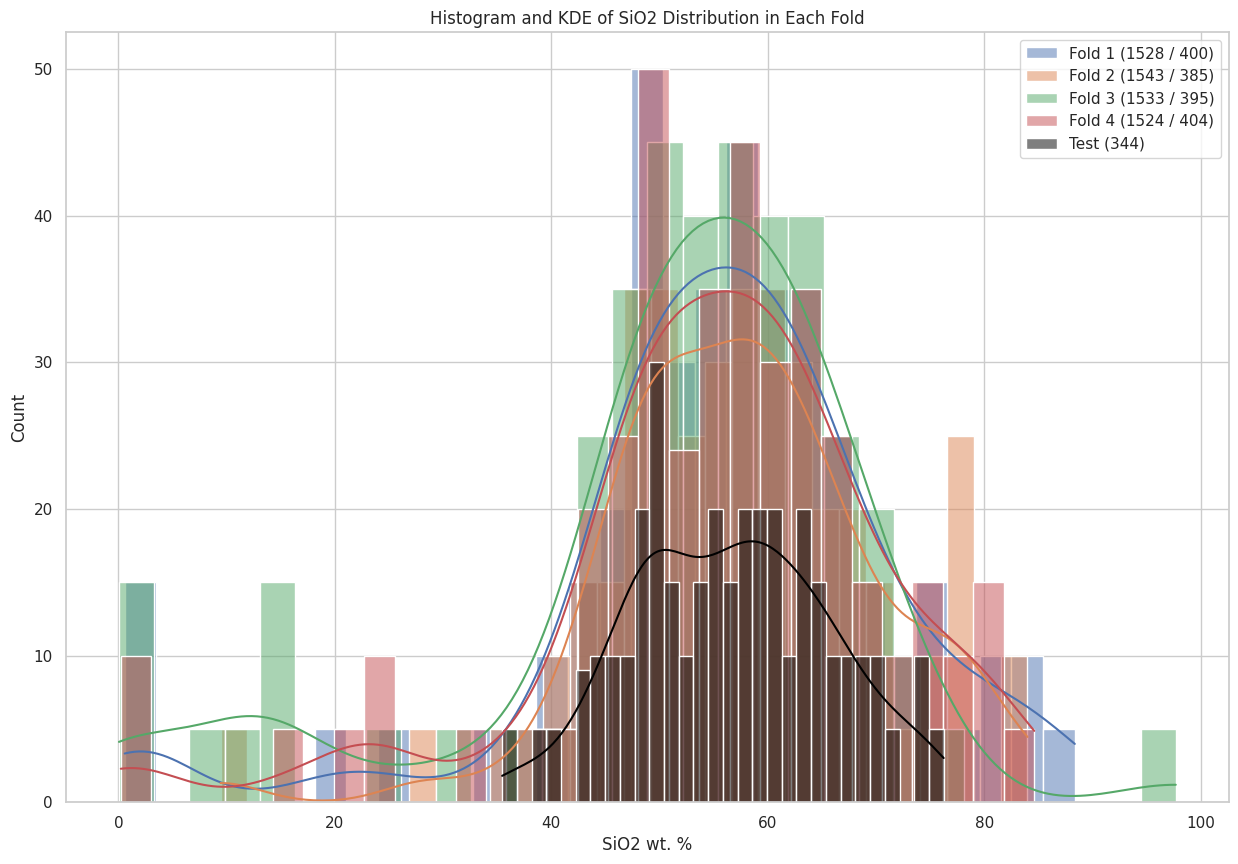
\includegraphics[width=\textwidth]{images/histogram_kde_plot.png}
    \caption{Combined Histogram and \gls{kde} of \ce{SiO_2} Distribution in Each Fold. The y-axis represents the count of samples per bin, and the x-axis represents \ce{SiO_2} concentration. The notation in the legend indicates the amount of instances in the training/validation sets.}
    \label{fig:histogram_kde_plot}
\end{figure*}

Figure \ref{fig:histogram_kde_plot} combines the histograms and \gls{kde} curves of \ce{SiO_2} values from each fold and the full test set into a single plot, using different colors to represent each fold and the test set.
This visualization enables direct comparison of the distributions across the folds and the test set.

The combined histograms and \gls{kde} curves show a high degree of overlap, reinforcing the observation that the distributions are consistent across different folds and the test set.
The test set distribution closely follows the overall pattern observed in the folds, indicating that the test set is also representative of the overall dataset.
The presence of extreme values is evident in the tails of the distributions, particularly in the training folds.

\begin{figure*}[h!]
    \centering
    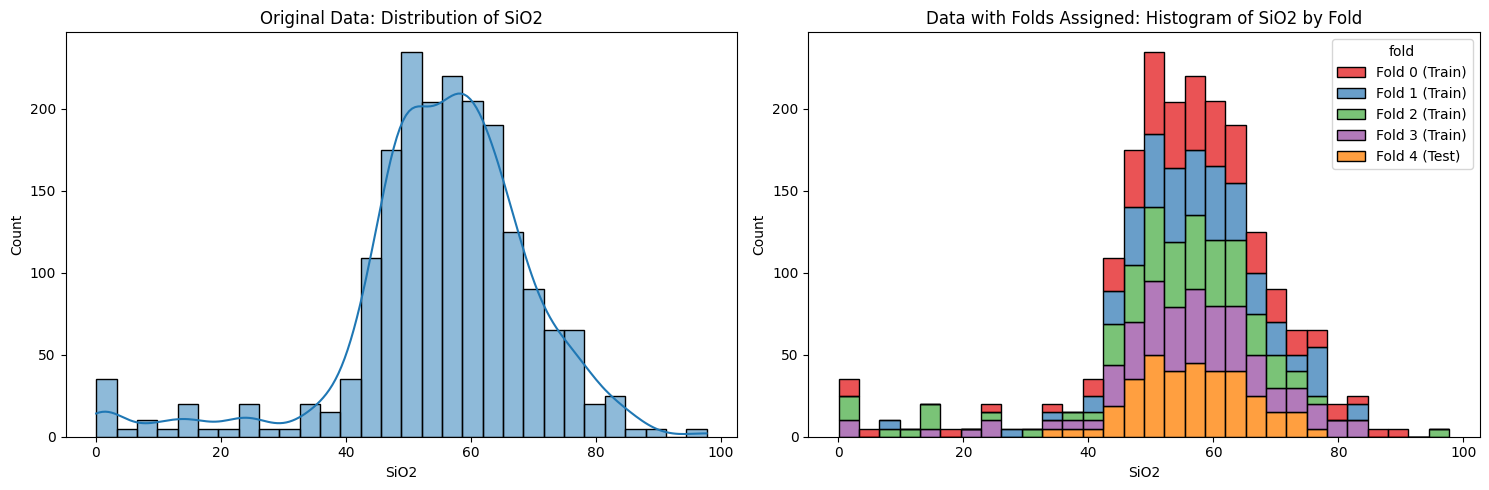
\includegraphics[width=\textwidth]{images/original_and_post_fold.png}
    \caption{Distribution of \ce{SiO_2} concentrations before and after fold assignment. The left plot shows the original distribution of \ce{SiO_2}, while the right plot shows the distribution with folds assigned, color-coded to indicate the different folds.}
    \label{fig:original_and_post_fold_plot}
\end{figure*}

Figure \ref{fig:original_and_post_fold_plot} contrasts the distribution of \ce{SiO_2} concentrations before and after the data partitioning process.
The left plot displays the original distribution of \ce{SiO_2} concentrations in the full dataset.
The right plot presents the distribution with assigned folds, using different colors to denote each fold.
This visualization highlights how the partitioning strategy maintains the overall data distribution while ensuring balanced representation across folds.